\titreTD{\thenumTD}{Recouvrements entre Orbitales Atomiques}

%##########################################################################
% NOTION DE RECOUVREMENT 
%##########################################################################

\textit{Pour se pr\'eparer \`a ces exercices, on pourra rappeler les sch\'emas des orbitales s, $p_x$, $p_y$, $p_z$ selon un rep\`ere impos\'e}.


\exo{D\'efinition}
\begin{enumerate}[\bf 1)]
\item   Rappelez l'expression du recouvrement $S_{ab}$, entre une orbitale $ \chi_a(r,\theta,\phi)$, et  $\chi_b(r,\theta,\phi)$.
\item  Que vaut exactement cette int\'egrale si $ \chi_a(r,\theta,\phi)=\chi_b(r,\theta,\phi)=\chi(r,\theta,\phi)$.
\item    Montrez graphiquement que les orbitales $2s_A$ et $2p_{z_{A}}$ (centr\'ee sur le m\^eme atome A), ont un recouvrement nul. Expliquez.
%\item    A quoi correspond la combinaison  $2s_A+2p_{z_{A}}$~? 
\end{enumerate} %\exo{Variation du Recouvrement avec la distance}
\exo{Recouvrement d'orbitales atomiques}
\label{exo_s}
Dans une mol\'ecule A$-$B, on \'etudie le recouvrement entre 2 orbitales atomiques, l'une centr\'ee sur un atome A, l'autre sur  B. Pour l'ensemble de cet exercice, les axes sont d\'efinis selon la figure du rep\`ere ci-dessous (l'axe internucl\'eaire d\'efinit l'axe Oz, et $x$ est dans le plan de la feuille, vers le haut). 
\\

Pour chaque cas propos\'e,

\begin{minipage}[c]{0.8\linewidth}
\begin{enumerate}[(i)] 
\item dessinez les orbitales en pr\'esence
\item indiquez la nature du recouvrement : $\sigma$, $\pi$ ou nul 
\item  pr\'ecisez s'il s'agit d'un recouvrement positif, n\'egatif ou nul
\end{enumerate} 
\end{minipage}
\begin{minipage}[l]{0.1\linewidth}     
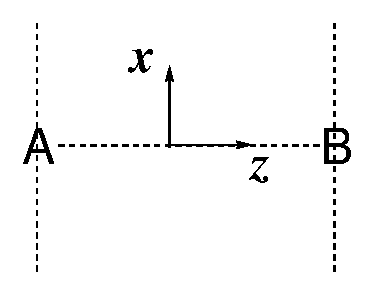
\includegraphics[scale=0.4]{figure/AB_repere.eps}\\   
Rep\`ere
\end{minipage}

\vspace{0.3cm}

\begin{minipage}[c]{0.5\linewidth}
\begin{enumerate}[\bf 1)]
\item $+2p_{x\textsc{a}}\ \, |+\,2p_{x\textsc{b}}$ 
\item $+2p_{z\textsc{a}}\ \, |-\,2p_{z\textsc{b}}$ 
\item $\ \, +2s_\textsc{a}\ \, |+\,2s_\textsc{b}$ 
\item $\ \, +2s_\textsc{a}\ \, |+\,2p_{z\textsc{b}}$ 
\item $+2p_{x\textsc{a}}\ \, |+\,2s_\textsc{b}$ 
%\item $+3p_{y\textsc{a}}\ \, |-\,3p_{y\textsc{b}}$
%\item $-3p_{x\textsc{a}}\ \, |-\,3s_\textsc{b}$
%\item $-2p_{x\textsc{a}}\ \, |-\,3p_{x\textsc{b}}$
\end{enumerate} 
\end{minipage} \hfill
\begin{minipage}[c]{0.5\linewidth}
 \textbf{Exemple :}  $+2s_\textsc{a}\ |-\,2s_\textsc{b}$
\begin{enumerate}[~~(i)] 
\item    Dessin~:\\[-0.3cm] 

   \  \  \  \  \   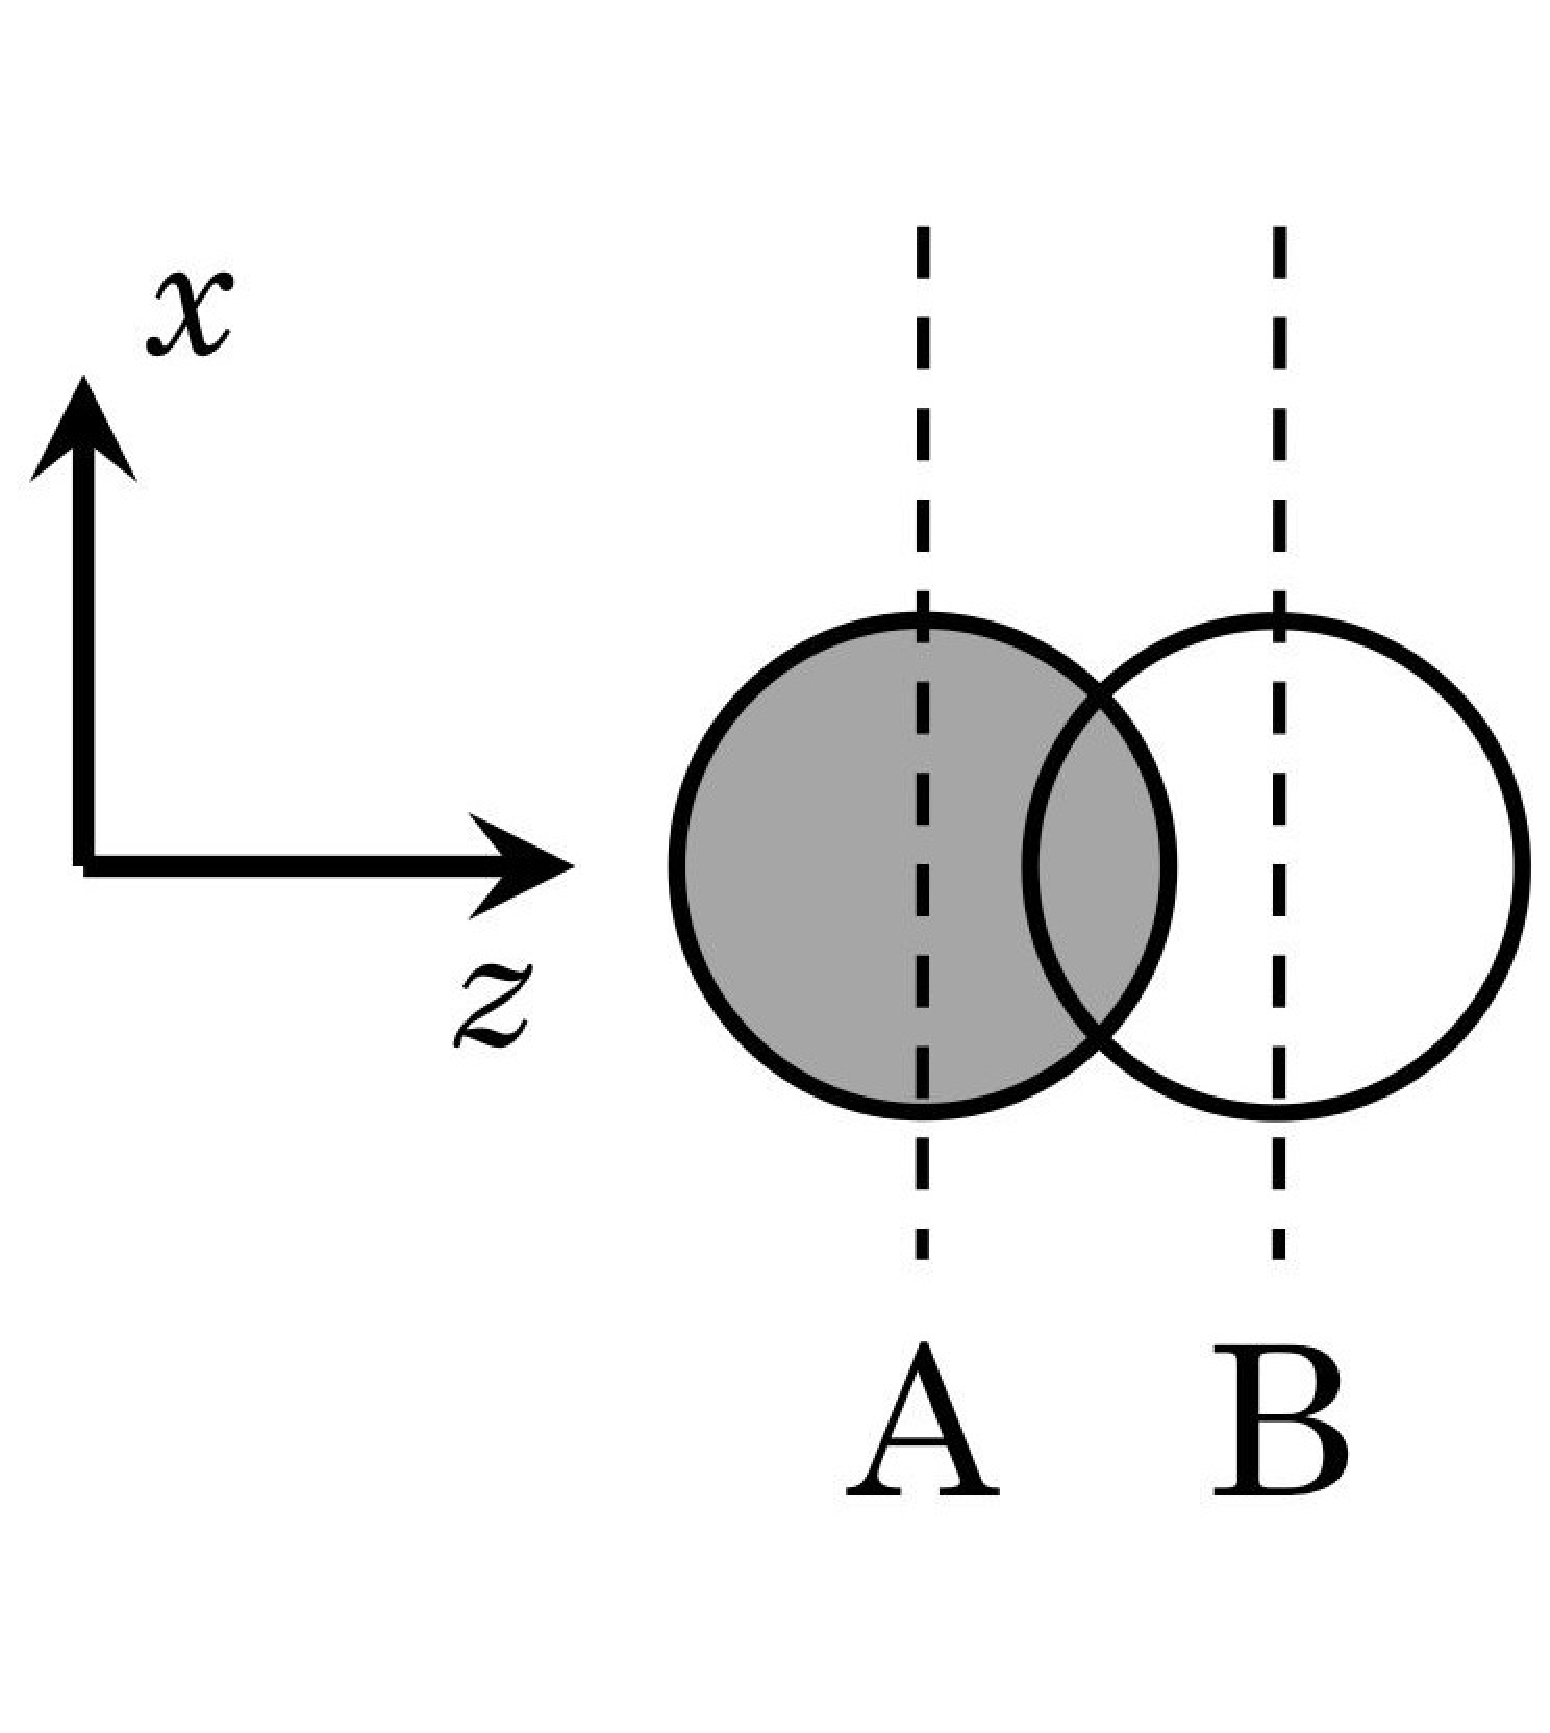
\includegraphics[scale=0.09]{figure/interactionOA.eps}
\item       Recouvrement axial, donc $\sigma$
\item       Recouvrement <0 car de phase $\neq $
\end{enumerate} 
\end{minipage}

%--------------------------------------------------------------------------
\exo{Recouvrement entre orbitales}

Les dessins des orbitales donnent la forme g\'en\'erale du volume o\`u l'\'electron
a le plus de chance de se trouver. M\^eme quand ces orbitales ne se touchent pas
graphiquement, on a un recouvrement.

\begin{enumerate}
\item On consid\`ere un atome qui se rapproche (suivant l'axe $z$) d'un atome de carbone.
Dessiner l'allure de l'\'evolution du recouvrement entre les diff\'erentes orbitales
pour $z \in ]-\infty;+\infty[$.

%%FIGURE
\vspace{-0.3cm}
\begin{center}
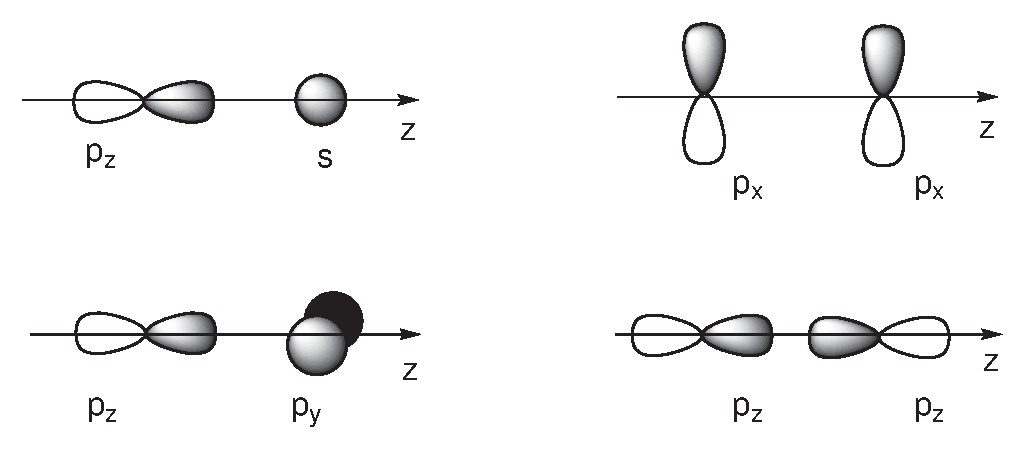
\includegraphics[width=8.0cm]{figure/overl1.eps}
\end{center}

\item On se place dans le cadre d'un recouvrement entre une orbitale de type \textit{s}
sur un atome et une orbitale de type \textit{p} sur un autre atome, situ\'e \`a proximit\'e
l'un de l'autre de sorte qu'il existe un recouvrement non nul si l'orientation de l'orbitale
\textit{p} est favorable.

\begin{enumerate}
\item Classer par ordre de recouvrement croissant les situations suivantes.
%%FIGURE
\vspace{-0.3cm}
\begin{center}
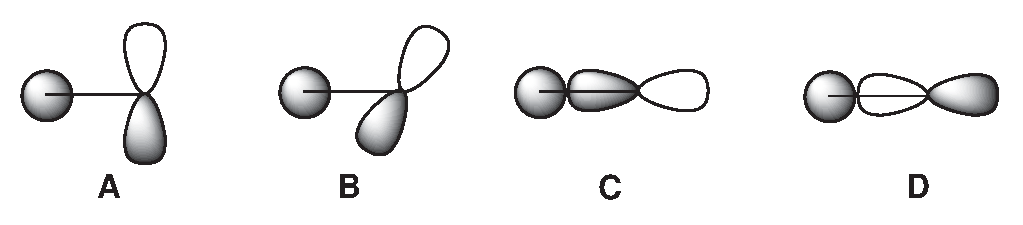
\includegraphics[width=8.0cm]{figure/overlangle.eps}
\end{center}

\item On appellera dans la suite $\alpha$ l'angle entre la direction internucl\'eaire et la
direction de l'orbitale (donn\'ee par la direction de sa phase sombre)~:

%%FIGURE
\vspace{-0.3cm}
\begin{center}
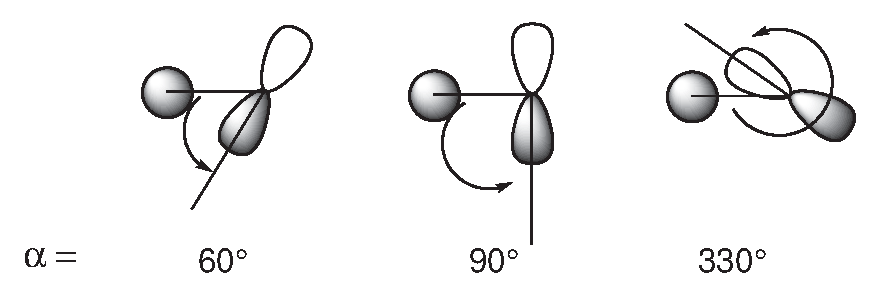
\includegraphics[width=7.5cm]{figure/overlalpha.eps}
\end{center}

Dessiner les situations \`a $\alpha  = 0^o, \ 180^o, \  270^o$.
Donner l'allure du recouvrement (toujours \`a distance constante) entre l'orbitale de type
\textit{s} et cette orbitale de type \textit{p} en fonction de l'angle $\alpha$ entre 0$^o$ et 360$^o$.

\end{enumerate}
\end{enumerate}

\exo{Matrice de recouvrement}

Dirac a propos\'e la notation suivante pour le recouvrement $S_{ij}$ 
entre deux orbitales $\chi_i$ et $\chi_j$~:

\[
S_{ij} = \langle \chi_i | \chi_j \rangle
\]

Dans cet exercice le rep\`ere est defini de la mani\`ere suivante~:

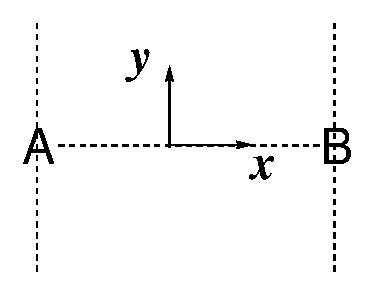
\includegraphics[width=2cm]{figure/AB_repere_yx.eps}

\begin{enumerate}

\item Sur un seul atome A, que vaut le recouvrement dans les cas suivants~:
\begin{enumerate}
\item $\chi_i = 1s_\textsc{a}$ et $\chi_j = 1s_\textsc{a}$~;
\item $\chi_i = 2s_\textsc{a}$ et $\chi_j = 2s_\textsc{a}$~;
\item $\chi_i = 2s_\textsc{a}$ et $\chi_j = 2p_{x\textsc{a}}$~;
\end{enumerate}

\item Pour deux atomes, A et B, s\'epar\'es d'une distance de liaison 
(environ 1.0-2.0~\AA), que vaut le recouvrement dans les cas suivants~: 
\begin{enumerate}
\item $\chi_i = 1s_\textsc{a}$ et $\chi_j = 1s_\textsc{b}$~;
\item $\chi_i = 2s_\textsc{a}$ et $\chi_j = 2s_\textsc{b}$~;
\item $\chi_i = 2s_\textsc{a}$ et $\chi_j = 2p_{x\textsc{b}}$~;
\end{enumerate}

\item Remplissez le tableau suivant, qu'on appelle la matrice recouvrement~:

\begin{tabular}{|c||c|c|c|c|c|}
\hline
                   & $2s_\textsc{a}$ & $2s_\textsc{b}$ & $2p_{x\textsc{b}}$ & $2p_{y\textsc{b}}$ & $2p_{z\textsc{b}}$ \\
\hline\hline
$2s_\textsc{a}$     &&&&& \\ \hline
$2s_\textsc{b}$     &&&&& \\ \hline
$2p_{x\textsc{b}}$  &&&&& \\ \hline
$2p_{y\textsc{b}}$  &&&&& \\ \hline
$2p_{z\textsc{b}}$  &&&&& \\ \hline
\end{tabular}


\end{enumerate}
